\documentclass[dvipdfm]{standalone}
\usepackage{tikz}
\usetikzlibrary{arrows,positioning,automata,shadows,fit,shapes}
\begin{document}
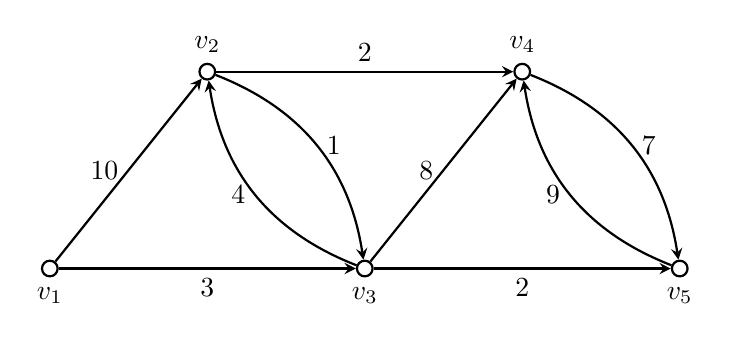
\begin{tikzpicture}
[nodedecorate/.style={shape=circle,inner sep=2pt,draw,thick},%
  arrowdecorate/.style={->,>=stealth,thick}]
%% nodes or vertices
\foreach \nodename/\x/\y/\direction/\navigate in {
  v_1/0/0/below/south, v_2/2/2.5/above/north, v_3/4/0/below/south,
  v_4/6/2.5/above/north, v_5/8/0/below/south}
{
  \node (\nodename) at (\x,\y) [nodedecorate] {};
  \node [\direction] at (\nodename.\navigate) {$\nodename$};
}
%% edges or lines
\path
\foreach \startnode/\endnode/\direction/\weight in {
  v_1/v_2/left/10, v_1/v_3/below/3, v_2/v_4/above/2, v_3/v_4/left/8,
  v_3/v_5/below/2}
{
  (\startnode) edge[arrowdecorate] node[\direction]{$\weight$} (\endnode)
}
\foreach \startnode/\endnode/\direction/\weight in {
  v_3/v_2/left/4, v_2/v_3/right/1, v_4/v_5/right/7, v_5/v_4/left/9}
{
  (\startnode) edge[arrowdecorate,bend left] node[\direction]{$\weight$} (\endnode)
};
\end{tikzpicture}
  \end{document}
